\documentclass[12pt,a4paper,leqno]{report}

\usepackage[T1]{fontenc}
\usepackage[english]{babel}
\usepackage{amsthm}
\usepackage{amsfonts}
\usepackage{amsmath}
\usepackage{amssymb}
\usepackage{tikz}
\usepackage{listings}

\newcommand{\R}{\mathbb{R}}
\newcommand{\C}{\mathbb{C}}
\newcommand{\Q}{\mathbb{Q}}
\newcommand{\N}{\mathbb{N}}
\newcommand{\No}{\mathbb{N}_0}
\newcommand{\Z}{\mathbb{Z}}
\newcommand{\diam}{\operatorname{diam}}

\theoremstyle{plain}
\newtheorem{equa}[equation]{Equation}
\newtheorem{lem}[equation]{Lemma}
\newtheorem{prop}[equation]{Proposition}
\newtheorem{cor}[equation]{Corollary}

\theoremstyle{definition}
\newtheorem{defi}[equation]{definition}
\newtheorem{conj}[equation]{Conjecture}
\newtheorem{example}[equation]{Example}
\theoremstyle{remark}
\newtheorem{note}[equation]{Note}

\pagestyle{plain}
\makeatletter
\renewcommand{\@seccntformat}[1]{}
\makeatother
\setcounter{page}{1}
\addtolength{\hoffset}{-1.15cm}
\addtolength{\textwidth}{2.3cm}
\addtolength{\voffset}{0.45cm}
\addtolength{\textheight}{-0.9cm}

\graphicspath{ {../figures/} }

\title{Data Analytics 2 - Market Basket Analysis}
\author{Tuomo Kareoja}
\date{}

\begin{document}

\maketitle

\begin{table}[h!]
  \begin{center}
    \begin{tabular}{l|c|r}
      \textbf{Version Number} & \textbf{Changes} & \textbf{Date} \\
      \hline
      0.5 & Basic structure, some text and plots & 16.09.2019\\
      1.0 & Finished text and plots & 17.09.2019\\
    \end{tabular}
  \end{center}
\end{table}

\newpage

\section{Main Takeaways}


\begin{enumerate}
    
    \item Although in most product categories Blackwell and Electronidex fit together nicely by offering products in different categories or
    product in different price ranges, with pc:s, displays and tablets there is considerable overlap. This is worrying as these 3
    categories create 45 \% of Blackwell's profits. All in all around 50 \% of our profits come from products that
    overlap with Electronidex product line. A better analysis could be performed if we also had the profits per product
    also from Electronidex. If we had this information we could make rough estimates of the profits of the
    possible combined company.

    \item Electronidex has a huge portfolio of over 4000 products and, as there are only slightly over 10000
    transactions with more than 1 unique product in the dataset, it is hard to find reliable connections for
    buying certain products together as most product appear only a couple of times in the transactions.
    Even if we add brand to the analysis the results are still uninteresting.
    More data would be needed to perform analysis on this level of detail.

    \item If we perform the market basket analysis at level of product categories, we find interesting
    connections between buying smartwatches, cameras and products of category other (these include
    a number of different products e.g. lamps with usb ports for charging other devices, connected
    thermostats etc.) and buying products belonging to the most profitable categories
    in Blackwell's product lineup: displays, tablets, pc:s, laptops, smartphones, printers and software.
    These associations offer strong cross selling possibilities as Blackwell does not itself
    offer any products in the predictive categories. A successful cross-selling of printers and
    software (where Electronidex offerings are lacking) would net Blackwell an estimated extra 5250 \$
    of yearly profits.
   
\end{enumerate}

\section{Blackwell Product Line Comparison to Electronidex Product Line}

Blackwell's two most profitable product categories are displays and game consoles. These two groups
create 55 \% of Blackwell's profits at the moment. After these two groups
there are 6 product groups that also contribute substantially, but that are not individually on the same
level of importance as the two biggest categories. These products create 41 \% of our profits.
Below is a breakdown of our profits by percentage by product category. Extended warranties are not included
in this plot as the data that we have from them is suspicious as it seems to have copy pasted values
between different warranties.

\bigskip
{
    \centering
    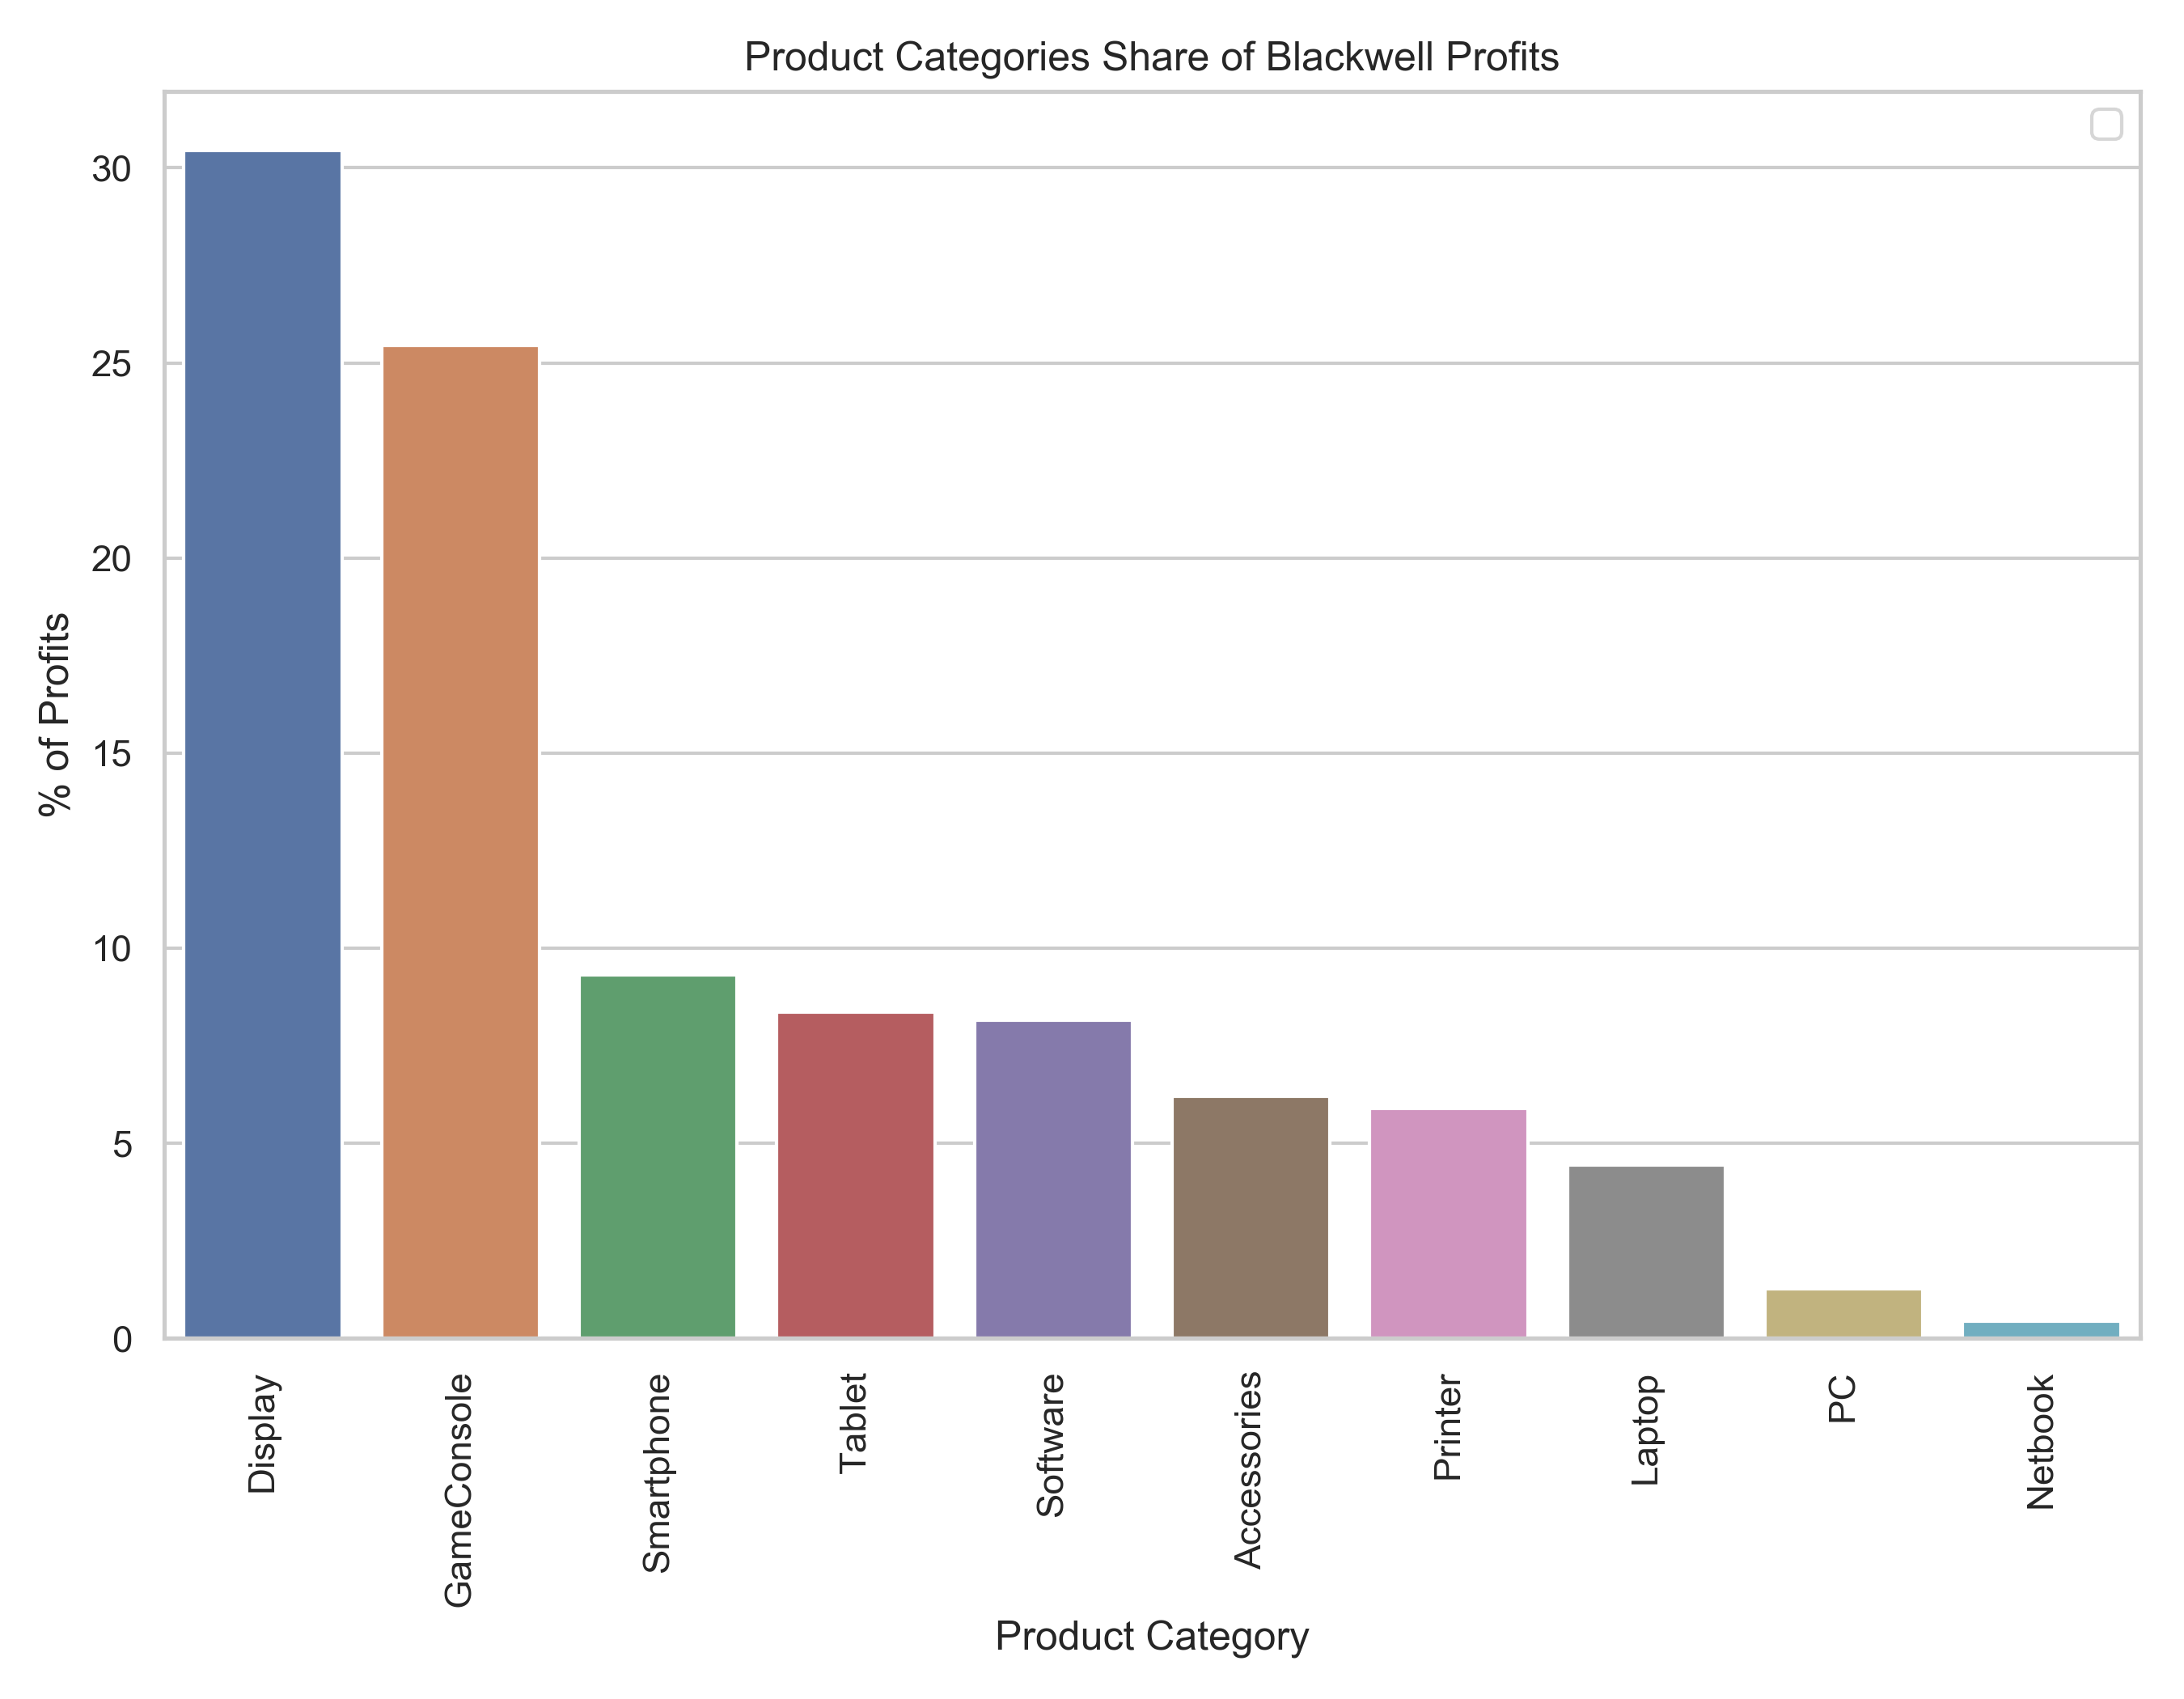
\includegraphics[width=\textwidth,height=\textheight,keepaspectratio]{blackwell_profits_share_by_product_category.png}
    \par
}
\bigskip

Next we look at the profits created from individual sales of our products. Below we have plotted our available
products sorted to product categories with their profit created per sold unit on the y-axis.
We see that our profits per product are actually quite consistent except for accessories
and one very high profit product in PC:s and another in Displays.
By comparing these to the breakdown of our profits per category we can come to the conclusion that to diversify
our profit making increasing our sales of PC:s, laptops, software, printers, tablets and smartphones would be
advisable. Especially PC:s, Laptops and Tablets offer big profits per sold product. We keep this in mind
when looking at what Electronidex has in their product lineup.

\bigskip
{
    \centering
    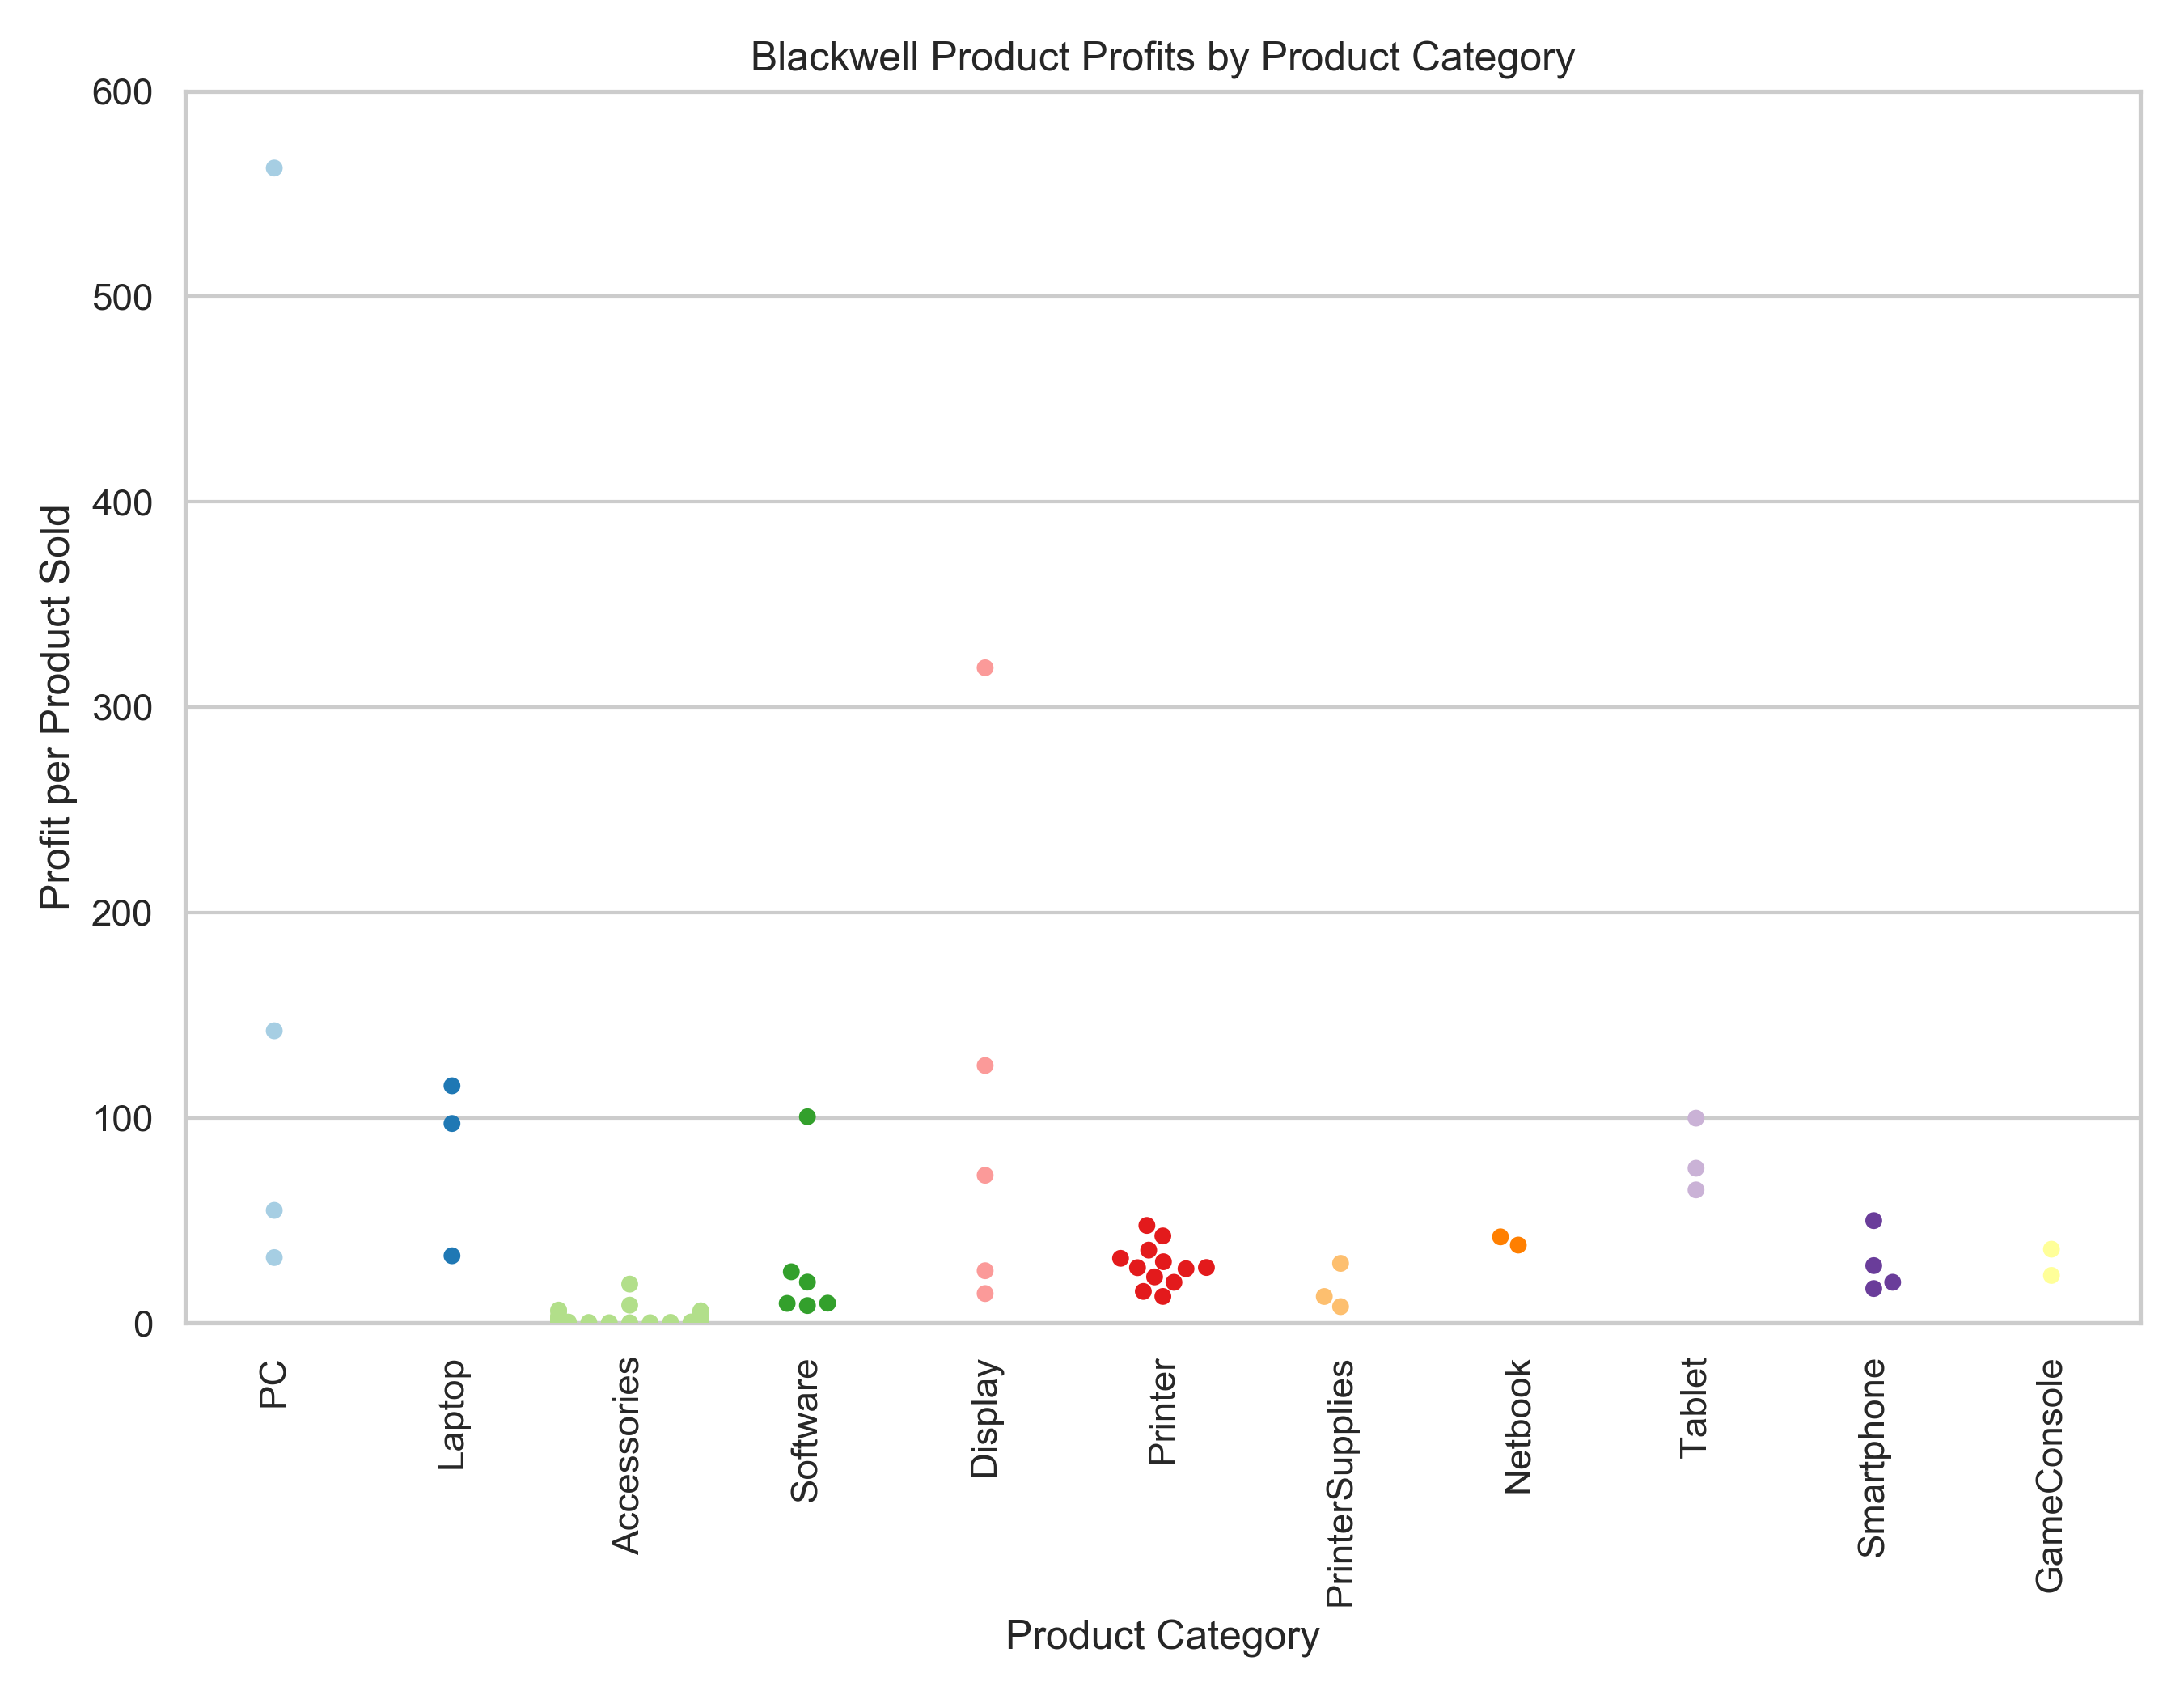
\includegraphics[width=\textwidth,height=\textheight,keepaspectratio]{blackwell_product_profitability_distribution_by_category.png}
    \par
}
\bigskip

Lets now see how our product lineup matches that of Electronidex. Below is a plot Blackwell's and Electronidex
products by product categories with their list prices (in Electronidex case we used the median price of sold items
to take into account how often there are discounts or other variation that might skew the real price away from list price).
Accessories have been left out this picture as there are too many products to visualize properly. Suffice to say
that in this category there is considerable overlap if we look at just the price and category, but
accessories is a difficult category to analyze as often these are related to just certain products and in these cases
if our products are not exactly the same there would be no overlap. Because of this reason we have left
accessories out from the following analysis. We should also keep in mind that accessories make up only 6 \%
of Blackwell's current profits.

\bigskip
{
    \centering
    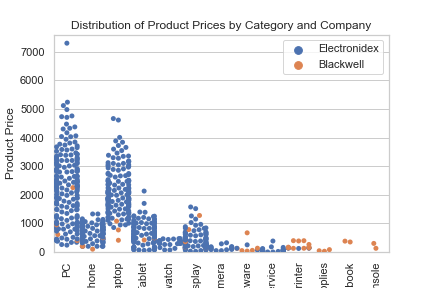
\includegraphics[width=\textwidth,height=\textheight,keepaspectratio]{product_prices_distribution_by_category_and_company.png}
    \par
}
\bigskip

We see that Electronidex has a very large product lineup that dwarfs ours.
Going trough each category we can divide the categories into ones that have little or no overlap, ones that have overlap,
but our products are differentiated by price, and ones where there is considerable overlap:

\begin{description}
   \item [No overlap:] smartwatch, camera, software, service, printer, printer supplies, netbook, game console
   \item [Overlap, but different prices:] smartphone, laptop
   \item [Overlap, no price difference:] PC, tablet, display
\end{description}

The categories that don't overlap and that have don't have any offerings from Blackwell include smartwatches, cameras
and services. These are product categories that would just extend our lineup if we acquired Electronidex.
The product categories that we have offering and Electronidex has none or only few include software, printers,
printer supplies, netbooks and game consoles. These product categories would not need to compete with Electronidex
offering and could benefit from cross-sales and make up 40 \% of our current profits.

The categories that have overlap, but where there is a price differentiation include smartphones and laptops.
In both of these categories our product add more options to the lower price range of these products. With laptops
our priciest model has similarly priced offerings from Electronidex product range but our two lower end products
would form a new low end offering to the combined product range. This is true somewhat also with smartphones
where are our cheapest phone is cheaper than any offering from Electronidex, but our other offerings
would be less clearly differentiated. Not including our highest end phone, this could still be ok, as the
low end offerings from Electronidex are more limited than their midrange offerings and our products would change this.
These two categories constitute 13 \% of our profits.

The categories where there is substantial overlap are PC:s, tablets and displays. Here our products
don't differentiate themselves from Electronidex offering by price. This means that our products
would possibly compete for the same customers. These categories form 40 \% of our current profits.

From this crude analysis we could say that roughly around 50 \% of our current profit sources don't
overlap with Electronidex offerings.

\section{Market Basket Analysis of Electronidex Transactions}

To get more insight to the customers of Electronidex and their buying habits a multilevel
market basket analysis was performed. The difficulty in this was that Electronidex has
such a huge product line that finding individual items that are often bought together
is very hard as most items appear in few transactions. This meant that adding brand level
and product category level to the analysis was necessary to find anything of interest and of
reasonable reliability.

\subsection{Product + Brand level}

Analyzing just the product level did not result in us finding any interesting
combinations of items as the number of individual products is too big find
items that would appear in enough transactions to make inference reliable.
Because of this, brand level was also added to the analysis by extracting
the first 3 letters from the product code.

Market basket analysis tries to find rules that predict the sale of a certain
item from buying of other items, e.g. buying a Asus laptop also includes extra
charger for the laptop. To limit the found rules only to reliable and meaningful
ones two statistic thresholds were used. Rules had appear in at least 1 \% of the
transactions with more than one unique items (104 transactions). This statistic
is called support and measures the applicability of the rule and also its
reliability as more observations mean that any found relationships
are not created just by a statistical fluke.
Second statistic that used to limit the rules was confidence which
measures which proportion of the transactions where the rule applies also
included buying the item that the rule predicts. This statistics is called
confidence and it was set to 0.4, so only rules where 40 \%
of the transactions that it covers led to buying the item predicted by the
rule were included. As our data only included transactions with more than
one unique items, the both confidence and support must be interpreted in this
context so they don't refer to proportions of all transactions, but only
transactions with more than one item.

Below we can see the plot of the 25 rules that met our criteria, by their
support and confidence. We can see that most of our rules have confidence
of 1 which means that these rules predicted the inclusion of the items
that they predict with perfect accuracy in transactions where they
apply. This seems good, but the amount of these rules also calls
into question the reliability of these finding: what are the real
world cases where buying a certain product or brand also leads
to buying certain other product or brand with absolute certainty?
The high confidence of the rules is an indication the available
data is not big enough to show real life uncertainties and we should
interpret the results with a pinch of salt.

\bigskip
{
    \centering
    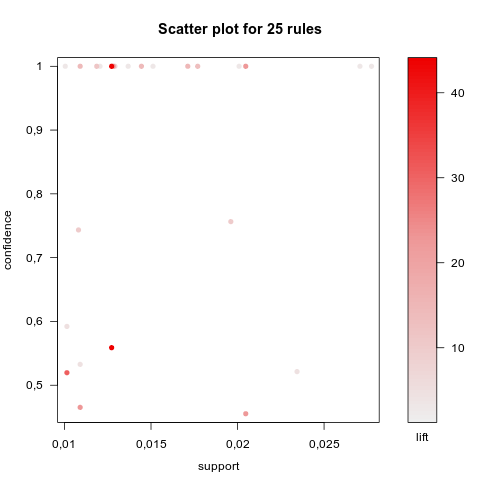
\includegraphics[width=\textwidth,height=\textheight,keepaspectratio]{apriori_brand_level_plot.png}
    \par
}
\bigskip

To show what do the rules predict, below is a graph of the rules that
shows the which products or groups of products predict buying other products.
The direction of the arrows tells the direction of the rule (buying certain item,
might predict buying certain other items, but not the other way around, e.g. charger is always
bought with the purchase of laptop, but laptop is not included in all purchases of the charger).
The size marks the support of the rule and the color marks the lift of the rule. Lift
tells us how many time more likely the product is to be bought when the rule applies
compared to how often the product is included in the transactions in general.

The interesting finding in this plot is the unsurprising finding that apple products (APP)
are often bought together with other Apple products. The other finding are more complicated
to explain and don't show clear general trends.

\bigskip
{
    \centering
    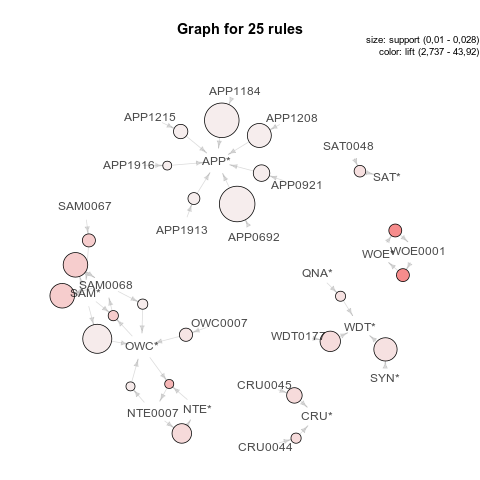
\includegraphics[width=\textwidth,height=\textheight,keepaspectratio]{apriori_brand_level_graph.png}
    \par
}
\bigskip


\subsection{Product Category Level}

To make the analysis more useful, the focus of the analysis was changed to product category level. Here we
tried to further limit the scope of the analysis by excluding rules that include accessories, service or extended
warranty as these categories are obviously related to other types of purchases and so don't offer much interesting
information. The rules that predict the sale of certain product categories from the sale of these items
are also probably getting the direction of causation wrong as a customer probably does not decide
to buy a bigger product after she made the decision to buy a warranty or accessory, but the other way around.
We also limited the rules so that only rules that predict sales in categories
display, laptop, smartphone, software, tablet, printer and pc
were included. These are the categories of products that Blackwell makes or could make profits. This
filtering made it easier to find categories that could have cross-selling potential. The support
threshold was set to 0.01 (104 transactions) and confidence to 0.4 as before.

Here we see that we have a clustering of rules where there is just enough support to pass
our filter and very high confidence value. In this case though compared to the analysis with
product and brands these rules are don't often have a confidence of 1 which seems more
realistic.

\bigskip
{
    \centering
    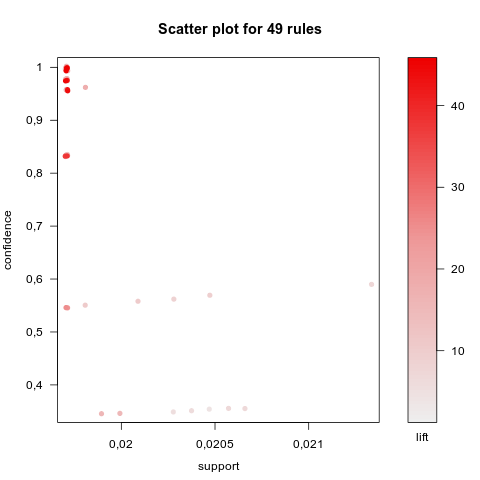
\includegraphics[width=\textwidth,height=\textheight,keepaspectratio]{apriori_product_category_level_plot.png}
    \par
}
\bigskip

If we look at the predictions of the rules we see that they included rules for all our target
categories and that they all predict sales in these categories from purchases of smartwatches, camera
or products in category other (these are not accessories, but more specialized products, like lamps with
integrated chargers) by themselves or in combination with the other two categories. This looks very interesting
as the predicting categories are all product categories that Blackwell does not offer. This means that we
are looking at transactions that might be made by buyers who Blackwell does not at the moment serve at all.
Of particular interest are the predictions for printers and software. These two categories are both categories
where the offering of Electronidex are very limited, but where Blackwell has numerous offerings. In these two
categories the rules have more predictive value measured from their lift that is shown with
color of the rules.

Although this found rules very interesting in possibly finding a customer segment that would
be a perfect cross-sale opportunity, the rules found here cover together only 280 transactions of the
over 10000 transactions with more than one unique product (2.3 \%). If we compare this number to the total
amount of transactions it is only 0.6 \%. This means that we might have found a good cross-sale
target group, but the size of this group is quite small.

\bigskip
{
    \centering
    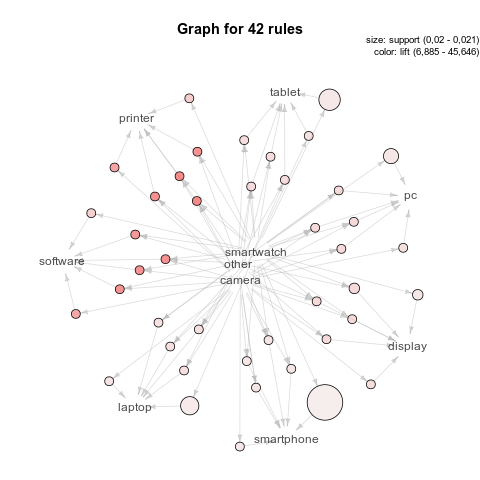
\includegraphics[width=\textwidth,height=\textheight,keepaspectratio]{apriori_product_category_level_graph.png}
    \par
}
\bigskip

To demonstrate possible extra profits lets suppose that the number of transaction with these
predictive product categories remains the same and that we could add a printer to 5 \% of the
1500 transactions that contains the predictive items, but in which there currently are no printers.
The 5 \% is quite a high number for this kind of thing, but we have to bear in mind that
printer offering from Electronidex are at the moment very limited so there is a possibility
to increase the sales substantially. Lets assume that these customers would buy a printer
in highest range of our products (50 \$ profit per printer). In this case we would make
1500 * 0.05 * 50 \$ = 3750 \$ extra yearly profits, which would increase the profits we make from
printers by 7 \%, but only increase our overall profits by 0.4 \%. If we would also succeed in
selling extra software to 5 \% of these transactions with a profit of 20 \$ per product (somewhere in the middle
of our software offerings profit) this would net us 1500 * 0.05 * 20 \$ = 1500 \$ yearly. This would
be an increase of 2 \% in our profits from software. With both these extra sales we would net
an extra 5250 \$ yearly, which would be an increase of 0.5 \% to our total profits.

These calculated increases are quite small and the problem of this market basket based analysis
is that it cannot answer our what would happen with our most profitable product categories: displays
and game consoles. The problem with displays is that, as we have demonstrate above, our products
are not clearly differentiated from Electronidex products and so it is very hard to assess if the
how combining are product lines would affect our sales as our products would compete with the
Electronidex offerings. With the game consoles the problem is more straight forward: as
Electronidex does not sell any game consoles we cannot assess if there is cross-selling
potential with a data driven approach like market basket analysis as there is no data.


\section{Suggested Next Steps}

The comparison of the product lines of Blackwell and Electronidex could be extended substantively if we had
information about the profit that different products create for Electronidex. If we had this information
we could compare our product lines so that we could see if there would be cases where we have offerings
in the same price range, but the products of one firm are more profitable. This would make it possible
to make some rough predictions of the profits in the cases that companies are merged with different
models of combining our product lines.

We could try to categorize the Electronidex product range with other available information to find product
categories that suitable sized. This would allow us to find more interesting patterns in the transactions
that would also be more reliable. The outcome of this kind of analysis is still highly uncertain and it is possible
that we would not find nothing of interest.

\end{document}
